\subsection{Finite Element Analysis - Bars and Trusses - Chapter 31
  (Kind of)}

In finite element methods as opposed to finite difference approaches
the bodies are broken up into nodes rather than discretized into equal
parts. These bodies can be one, two or even three dimensional objects
as shown in the figure below.

\begin{figure}[H]
  \begin{center}
    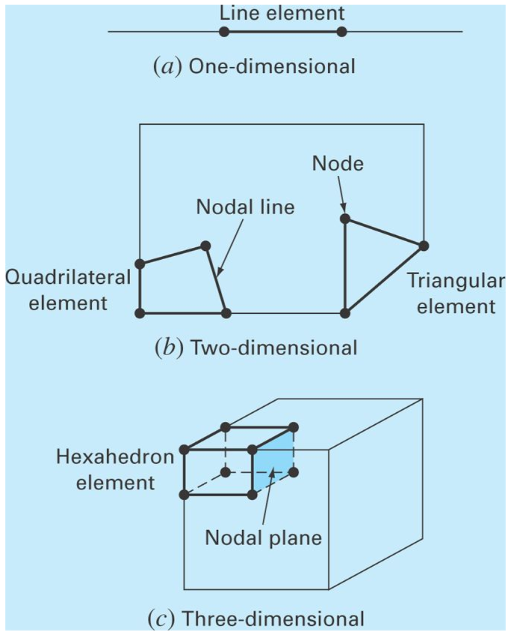
\includegraphics[height=0.5\textwidth,width=0.4\textwidth]{Graphics/cha9792x_3102_lg.jpg}
  \end{center}
\end{figure}

These nodes are not restricted to be linear and thus offer more
capabilities over finite difference methods. The chapters below will
begin with the derivation of a 1-D beam with examples to follow

\begin{enumerate}

\item {\bf Finite Element Analysis of a 2-Node Bar}

For the moment let's consider the one dimensional object. Typically
approximation functions are created to approximate the nodes such that

\beq\label{e:fea}
u(x) = a_0 + a_1x
\eeq

where $u(x)$ is whatever the independent variable can be and the
coefficients $a$ are constants to be solved for. When a
one-dimensional bar is split into different nodes we must enforce the
constraint that $u(x_1)=u_1$ is equal to $u(x_2)=u_2$ where $x_1$ and
$x_2$ are the coordinates of the nodes along the beam. This constraint
for a two node beam would yield the following two equations.

\beq
\begin{matrix}
u_1 = a_0 + a_1 x_1 \\
u_2 = a_0 + a_1 x_2
\end{matrix}
\eeq

These equations can be easily solved for using substitution or
Gaussian Elimination. 

\beq
\begin{matrix}
a_0 = \frac{u_1x_2-u_2x_1}{x_2-x_1} & a_1 = \frac{u_2-u_1}{x_2-x_1}
\end{matrix}
\eeq

These equations can then be further reduced by setting

\beq
N_1 = \frac{x_2-x}{x_2-x_1}
\eeq

and 

\beq
N_2 = \frac{x-x_1}{x_2-x_1}
\eeq

such that equation \ref{e:fea} becomes

\beq\label{e:shape}
u = N_1u_1 + N_2u_2
\eeq

The equation above is called a {\it shape function} and $N_1$ and
$N_2$ are called {\it interpolation functions}. The solution does not
seem very fancy however it leads to very interesting results in
differentiation and integration. For example, if equation
\ref{e:shape} is differentiated to obtain

\beq
\frac{du}{dx} = \frac{dN_1}{dx}u_1 + \frac{dN_2}{dx}u_2
\eeq

where

\beq
\begin{matrix}
\frac{dN_1}{dx} = -\frac{1}{x_2-x_1} & \frac{dN_2}{dx} = \frac{1}{x_2-x_1}
\end{matrix}
\eeq

Noting that $u_1$ and $u_2$ are not functions of x. The variable
$u(x)$ is a function of x but $u_1$ and $u_2$ are constants w.r.t
x. Substituting this into the equation for the derivative yields  

\beq\label{e:fea_deriv}
\frac{du}{dx} = \frac{u_2-u_1}{x_2-x_1}
\eeq

which is simply the slope of the line. Similarly, the integral of
$u(x)$ can be expressed as

\beq
\int\limits_{x_1}^{x_2}u~dx = \int\limits_{x_1}^{x_2}N_1u_1 + N_2u_2~dx = \frac{u_1+u_2}{2}(x_2-x_1)
\eeq

Close inspection reveals that the equation above is simply the
trapezoidal rule. Thus, using shape functions create a simple equation
for both the derivative and the integral. Something that can be used
when creating the differential equations for governing bodies. The
task then becomes to solve for the value of $u(x)$ at all node
locations. 

  \item {\bf Stiffness Matrix for a Bar Element}

As a first example, let's consider the uniform bar being loaded axially
below. If this bar is discretized into N or more beads the problem
becomes considerably more complex than if the bar was simply
discretized into two nodes (the left and right dots labeled 1 and
2). In this fashion the loads are computed at 1 and 2 and are assumed
to be uniform throughout the entire member.

  \begin{figure}[H]
     \begin{center}
       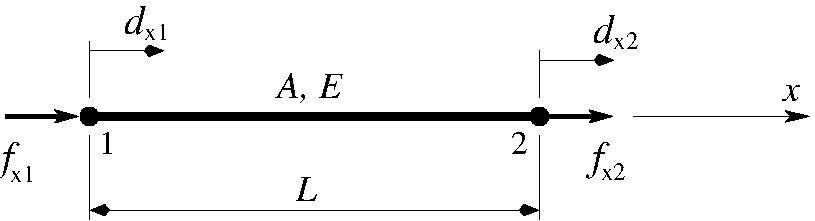
\includegraphics[height=0.15\textwidth,width=0.5\textwidth]{Graphics/L06_F1.pdf}
     \end{center}
   \end{figure}

  Consider again the uniform prismatic bar element of length $L$,
  cross-sectional area $A$ and Young's modulus $E$. Assume for the
  moment this bar is just a uniform bar and can resist only axial
  load, thus nodes are allowed to displace only in the 
  axial direction. The displacement-force relation and the equation of static
  equilibrium in the $x$-direction are respectively given by Hooke's
  law where Force = stiffness * displacement
  
  \begin{equation}
    k(d_{x2} - d_{x1}) = f_{x2}
  \end{equation}
  
  where $k=EA/L$ is the axial stiffness constant, and

  \begin{equation}
    f_{x1} = -f_{x2}  
  \end{equation}

  If put into matrix form with the forces on the right hand side the
  equations become

  \begin{equation}
    k\begin{bmatrix} 1   &-1   \\  -1
        &1 \end{bmatrix} \begin{Bmatrix} d_{x1} \\ d_{x2} \end{Bmatrix}
      = \begin{Bmatrix} f_{x1} \\ f_{x2} \end{Bmatrix}
  \end{equation}

  As a result, the stiffness matrix for a bar element can be found as

  \begin{equation}\label{e:singlebar}
    \left[K_{(e)}\right] = k\left[ \begin{matrix} 1   &-1   \\  -1  &1 \end{matrix} \right]
  \end{equation}

  \item {\bf Stiffness Matrix for a Bar Assemblage}

    With the stiffness matrix of one bar known it is now possible to
    create a stiffness matrix of an entire assemblage. The structure
    stiffness matrix $[K]$ may be obtained by assembling
    $\left[K_{(e)}\right]$ of $n$ individual bar elements.

    \begin{equation}
      [K] = \sum\limits_{e=1}^n \left[K_{(e)}\right]
    \end{equation}

    For example, consider the bar below with two elements connected to
    a wall. 

    \begin{figure}[H]
      \begin{center}
        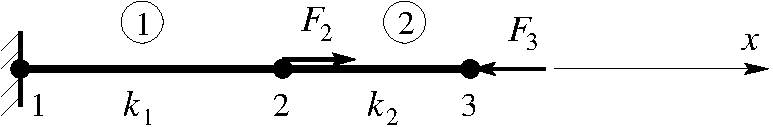
\includegraphics[height=0.1\textwidth,width=0.5\textwidth]{Graphics/L06_F2.pdf}
      \end{center}
    \end{figure}

    The stiffness matrices can be written for both bars using equation \ref{e:singlebar}.

    \begin{equation}
      \left[K_{(1)}\right] = k_1 \,
      \left[ \begin{array}{rr}
          1  &-1   \\
          -1  &1
        \end{array} \right]
      \begin{Bmatrix}
        d_{x1} \\ d_{x2}
      \end{Bmatrix}
      \hspace{3cm}
      \left[K_{(2)}\right] = k_2 \,
      \left[ \begin{array}{rr}
          1  &-1   \\
          -1  &1
        \end{array} \right]
      \begin{Bmatrix}
        d_{x2} \\ d_{x3}
      \end{Bmatrix}
    \end{equation}

    In order to obtain the total stiffness matrix $[K]$ the 2x2
    systems must be expanded to 3x3 systems.
    
    \begin{equation}
      \left[K_{(1)}\right] =
      \left[ \begin{array}{rrr}
          k_1  &-k_1  & 0   \\
          -k_1  & k_1  & 0   \\
          0    & 0    & 0
        \end{array} \right]
      \begin{Bmatrix}
        d_{x1} \\ d_{x2} \\ d_{x3}
      \end{Bmatrix}
      \hspace{3cm}
      \left[K_{(2)}\right] =
      \left[ \begin{array}{rrr}
          0    & 0    & 0   \\
          0    & k_2  &-k_2 \\
          0    &-k_2  & k_2
        \end{array} \right]
      \begin{Bmatrix}
        d_{x1} \\ d_{x2} \\ d_{x3}
      \end{Bmatrix}
    \end{equation}

    \begin{equation}
      \to ~~~
          [K] = \left[K_{(1)}\right] + \left[K_{(2)}\right] =
          \left[ \begin{array}{ccc}
              k_1  &-k_1        & 0   \\
              -k_1  & (k_1+k_2)  &-k_2 \\
              0    &-k_2        & k_2
            \end{array} \right]
          \begin{Bmatrix}
            d_{x1} \\ d_{x2} \\ d_{x3}
          \end{Bmatrix}
    \end{equation}
    
    The full system of equations is then simply $[K]\vec{d} = \vec{F}$

    \begin{equation}
    \left[ \begin{array}{ccc}
        k_1  &-k_1        & 0   \\
        -k_1  & (k_1+k_2)  &-k_2 \\
        0    &-k_2        & k_2
      \end{array} \right]
    \begin{Bmatrix}
      d_{x1} \\ d_{x2} \\ d_{x3}
    \end{Bmatrix} = \begin{Bmatrix} R_{x1} \\ F_2
      \\ -F_3 \end{Bmatrix}
    \end{equation}

    The unknowns in the equation above are the displacements and the
    reaction force $R_{x1}$. In this example, $F_1$ and $F_2$ are
    known forcing functions. Even with these two values there are
    still 4 unknowns and only 3 equations. The last equation is
    obtained by using the boundary conditions of the system. This is
    the fact that the beam cannot deflect at the attachment point
    1. Thus $d_{x1} = 0$. Using this result the systems of equations
    reduces to 

    \begin{equation}
      \left[ \begin{array}{cc}
          (k_1+k_2)  &-k_2 \\
          -k_2       & k_2
        \end{array} \right]
      \left\{ \begin{array}{c}
        d_{x2}  \\ d_{x3}
      \end{array} \right\} =
      \left\{ \begin{array}{r}
        F_2  \\ -F_3
      \end{array} \right\}
    \end{equation}

    This system is in the form $A\vec{x} = \vec{b}$ and can now be
    easily solved by any computer program. Since the system is 2x2 it
    can also be easily solved by hand. Knowing the values of
    $\vec{d}$, it is possible to obtain the tension/compression force
    of each bar

    \beq
    \left\{f_{(e)}\right\} = \left[ K_{(e)} \right] \, \left\{d_{(e)}\right\}
    \eeq
    
    For example bar 1 is given as

    \beq
    \left\{f_{(1)}\right\} = \left[ K_{(1)} \right] \, \left\{d_{(1)}\right\}
    \eeq

    \begin{equation}
    \left\{ \begin{array}{c} f_{x1} \\ f_{x2}  \end{array} \right\}
    = k_1 \,\left[ \begin{array}{rr}
        1  &-1   \\
        -1  &1
      \end{array} \right]
    \left\{ \begin{array}{c}
      d_{x1} \\ d_{x2}
    \end{array} \right\} 
    \end{equation}

    Remember though that $f_{x1} = -f_{x2}$.

    \item {\bf FEA of a Bar Example Problem}

      Determine the nodal displacements, the forces in each
      element, and the reactions. Let ($E_{st} = 200$ GPa, $A_{st} = 4 \times
      10^{-4}$ m$^2$, $E_{al} = 70$ GPa, $A_{al} = 2 \times 10^{-4}$ m$^2$).
      
      \begin{figure}[H]
        \begin{center}
          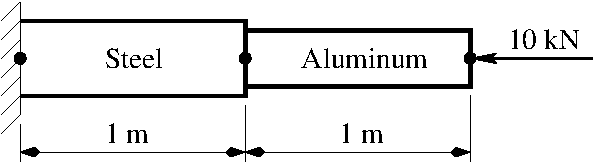
\includegraphics[height=0.1\textwidth,width=0.5\textwidth]{Graphics/L06_F3.pdf}
        \end{center}
      \end{figure}      

      \begin{enumerate}
        \item Displacements of nodes 2 and 3
          \beq
          \left[K_{(1)}\right] = k_1 \,
          \left[ \begin{array}{rr}
              1  &-1   \\
              -1  &1
            \end{array} \right] \hspace{3cm}
          \left[K_{(2)}\right] = k_2 \,
          \left[ \begin{array}{rr}
              1  &-1   \\
              -1  &1
            \end{array} \right]
          \eeq
          where
          \vspace{-1cm}
          \begin{eqnarray}
            k_1 &=& \frac{E_{st}A_{st}}{L} = \frac{(200 \times 10^6)
              (4 \times 10^{-4})}{1} = 8 \times 10^4 \mbox{ kN/m}  \nonumber \\
            k_2 &=& \frac{E_{al}A_{al}}{L} = \frac{(70 \times 10^6)
              (2 \times 10^{-4})}{1} = 14 \times 10^3 \mbox{ kN/m} \nonumber
          \end{eqnarray}

          Use of the BCs and loading conditions yields

          \beq
          \left[ \!\! \begin{array}{rcr}
              k_1  &-k_1       & 0    \\
              -k_1  &(k_1+k_2)  &-k_2  \\
              0    &-k_2       & k_2
            \end{array} \right] \!\!\!
          \left\{ \!\! \begin{array}{c}
            0 \\ d_{x2} \\ d_{x3}
          \end{array} \!\! \right\} \!\!=\!\!
          \left\{ \!\! \begin{array}{c}
            R_{x1} \\ 0 \\ -P
          \end{array} \!\! \right\}  ~~~ \mbox{or} ~~~
          10^3 \!\!\left[ \!\! \begin{array}{rrr}
              80  &-80  & 0   \\
              -80  & 94  &-14  \\
              0   &-14  & 14 
            \end{array} \right] \!\!\!
          \left\{ \!\! \begin{array}{c}
            0 \\ d_{x2} \\ d_{x3}
          \end{array} \!\! \right\} \!\!=\!\!
          \left\{ \!\! \begin{array}{c}
            R_{x1} \\ 0 \\ -10
          \end{array} \!\! \right\}  \label{Ex-3.2}
          \eeq

          Results:

          \beq
          10^3 \left[ \begin{array}{rr}
              94  &-14  \\
              -14  & 14 
            \end{array} \right]
          \left\{ \begin{array}{c}
            d_{x2}  \\ d_{x3}
          \end{array} \right\} =
          \left\{ \begin{array}{c}
            0  \\ -10
          \end{array} \right\} ~~~ \to ~~~
          \left\{ \begin{array}{c}
            d_{x2}  \\ d_{x3}
          \end{array} \right\} = 
          10^{-3} \left[ \begin{array}{rr}
              94  &-14  \\
              -14  & 14 
            \end{array} \right]^{-1}
          \left\{ \begin{array}{c}
            0  \\ -10
          \end{array} \right\}
          \eeq

          Thus,
          
          \beq
          \left\{ \begin{array}{c}
            d_{x2}  \\ d_{x3}
          \end{array} \right\} =
          10^{-4} \left\{ \begin{array}{c}
            -1.25  \\ -8.39
          \end{array} \right\} \mbox{ m} =
          \left\{ \begin{array}{c}
            -0.125  \\ -0.839
          \end{array} \right\} \mbox{ mm}
          \eeq

        \item Forces in each element: $\left\{f_{(e)}\right\} = \left[ K_{(e)} \right] \, \left\{d_{(e)}\right\}$

          \beq
          \mbox{Element 1:} ~~~
          \left\{ \begin{array}{c}
            f_1  \\ f_2
          \end{array} \right\} = 8 \times 10^4 \,
          \left[ \begin{array}{rr}
              1  &-1 \\
              -1  & 1
            \end{array} \right]
          \left\{ \begin{array}{l}
            d_{x1}=0  \\ d_{x2}=-1.25 \times 10^{-4}
          \end{array} \right\} =
          \left\{ \begin{array}{r}
            10 \\ -10
          \end{array} \right\} \mbox{ kN}
          \eeq

          \beq
          \mbox{Element 2:} ~~~
          \left\{ \begin{array}{c}
            f_2  \\ f_3
          \end{array} \right\} = 14 \times 10^3 \,
          \left[ \begin{array}{rr}
              1  &-1 \\
              -1  & 1
            \end{array} \right]
          \left\{ \begin{array}{l}
            d_{x2}=-1.25 \times 10^{-4} \\ d_{x3}=-8.39 \times 10^{-4}
          \end{array} \right\} =
          \left\{ \begin{array}{r}
            10 \\ -10
          \end{array} \right\} \mbox{ kN}
          \eeq

          Notice that in Element 1, $f_2 = -10 kN$ but in Element 2,
          $f_2 = 10 kN$. This is because the force $f_2$ is seen as
          compression for Element 1 and tension for Element 2. This is
          a direct consequence of Newton's 3rd Law.

        \item Reaction $R_{x1}$ (using the first equation in (\ref{Ex-3.2}))
          \beq
          R_{x1} = -k_1 \, d_{x2}  = (-8 \times 10^4)(-1.25 \times
          10^{-4}) = 10 \mbox{ kN}
          \eeq
      \end{enumerate}

    \item {\bf Introduction to Trusses} \label{s:trusses}

      Trusses as opposed to bars are not restricted to one
      dimension. That is, a truss is a system of interconnected bars
      who can still only support axial loading but in their local
      reference frame. A drawing of a 2 beam truss in 2-dimensions is
      shown below.  

      \begin{figure}[H]
        \begin{center}
          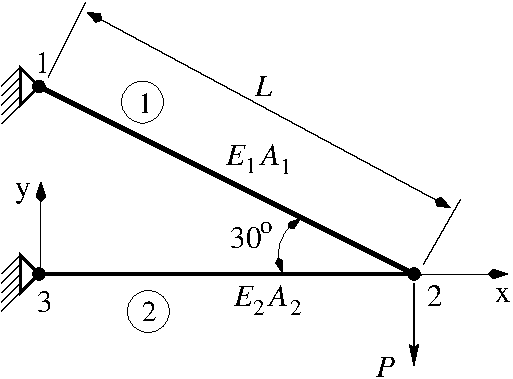
\includegraphics[height=0.2\textwidth,width=0.3\textwidth]{Graphics/L06_F5.pdf}
        \end{center}
      \end{figure}

      In the problem above Let $A_1=A_2=5$ in.$^2$, $E_1=E_2=10^6$
      psi, $L=100$ in., and $P=10$ kip (klbf). In order to solve for the displacement at node 2 the stiffness
      matrices of each member must be translated to a global inertial
      coordinate system. In the problems with 1-D beams the local body
      frame of each beam was identical to the global inertial
      frame. However in the 2D truss problem, each beam is rotated
      through an angle $\theta$ as shown by the problem below.

      \begin{figure}[H]
        \begin{center}
          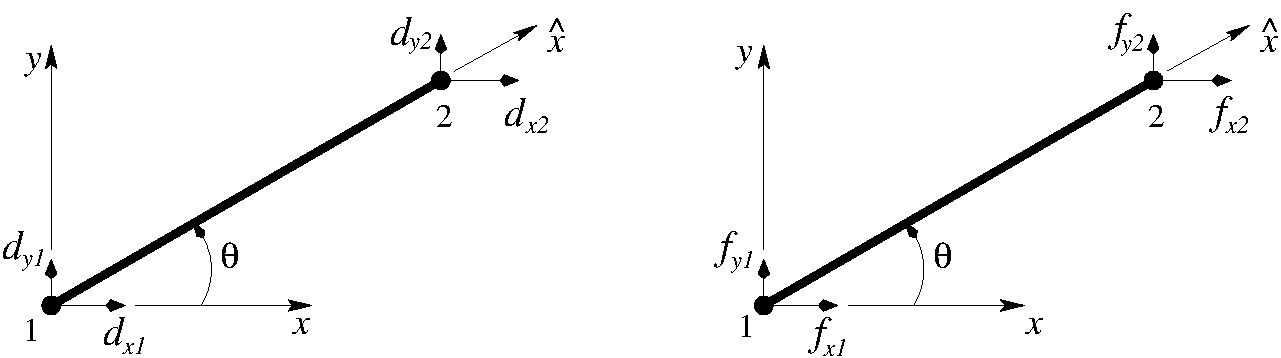
\includegraphics[height=0.2\textwidth,width=0.65\textwidth]{Graphics/L06_F4.pdf}
        \end{center}
      \end{figure}

      The nomenclature for the two
      frames is a superscript $[I]$ for 
      inertial and $[B]$ for body or beam frame. The first step is to
      write the stiffness in the local body frame as

      \beq
      \left[K_{(e)}^{[B]}\right] \, \vec{d_{(e)}}^{[B]} = \vec{f_{(e)}}^{[B]}
      \label{FE-eq-local}
      \eeq
      
      Note that this is a vector equation thus as long as the
      superscript [~~] is the same on all variables the equation is
      satisfied. This equation can also be written in component form as 

      \beq
      k \left[ \begin{array}{rr}
          1   &-1   \\
          -1   & 1
        \end{array} \right] \left\{
      \begin{array}{c}
        \delta_{x1} \\ \delta_{x2}
      \end{array}
      \right \} = \left\{
      \begin{array}{c}
        g_{x1} \\ g_{x2}
      \end{array}
      \right \}
      \eeq

      Notice that $\delta$ and $g$ are used to denote the components
      of displacement and force in the local body frame. Clearly there
      is a relationship between the body frame components and the
      inertial frame components. To do this a rotation matrix $T_{IB}$
      is used to rotate from one coordinate system to the other. This
      can be written as 

      \beq
      \vec{d_{(e)}}^{[I]} = \left[T_{IB}\right]\vec{d_{(e)}}^{[B]}
      \eeq

      The rotation matrix has the property of being an orthonormal
      basis in $R^N$ thus $T_{IB}^{-1} = T_{IB}^T = T_{BI}$. Thus the
      equation above can be written simply as 

      \beq
      \vec{d_{(e)}}^{[B]} = \left[T_{IB}^T\right]\vec{d_{(e)}}^{[I]}
      \label{e:inertialtobody}
      \eeq

      The derivation of $T_{IB}$ is left out for space but the reader
      is encouraged to consult his/her dynamics textbook on 2D rigid
      body rotations to obtain the $T_{IB}$ matrix below. It is
      advised not to just memorize this matrix and learn the steps to
      derive the matrix. 
      
      \beq
      \left[T_{IB}\right] = \begin{bmatrix} cos(\theta) & -sin(\theta)
        \\ sin(\theta) & cos(\theta) \end{bmatrix}
      \eeq

      If equation \ref{e:inertialtobody} is substituted into equation \ref{FE-eq-local}
      the equation becomes

      \beq
      \left[K_{(e)}^{[B]}\right] \, \left[T_{IB}^T\right]\vec{d_{(e)}}^{[I]} = \left[T_{IB}^T\right]\vec{f_{(e)}}^{[I]}
      \eeq
      
      Multiplying both sides of the equation by $T_{IB}$ yields

      \beq
      \left[T_{IB}^T\right] \left[K_{(e)}^{[B]}\right] \, \left[T_{IB}^T\right]\vec{d_{(e)}}^{[I]} = \vec{f_{(e)}}^{[I]}
      \eeq

      Notice then that all terms contain the superscript $[I]$ except
      for the stiffness matrix. This can be solved by substituting in
      the equation below.
      
      \beq
      \left[K_{(e)}^{[I]}\right] = \left[T_{IB}^T\right] \left[K_{(e)}^{[B]}\right] \, \left[T_{IB}^T\right]
      \eeq

      This equation relates the local body frame coordinate system for
      the global inertial coordinate system. Using this equation
      yields the final vector equation.

      \beq
      \left[K_{(e)}^{[I]}\right] \, \vec{d_{(e)}}^{[I]} = \vec{f_{(e)}}^{[I]}
      \eeq

      At this point the solution to the problem is identical to a 1D
      bar problem. Thus the example presented above is left as an
      exercise to the reader. Remember that in order to solve this the
      constraint that beams can only hold axial loads must be held. 
      
\end{enumerate}
